\appendix
\section{Appendix}

\begin{figure}[H]
    \centering
  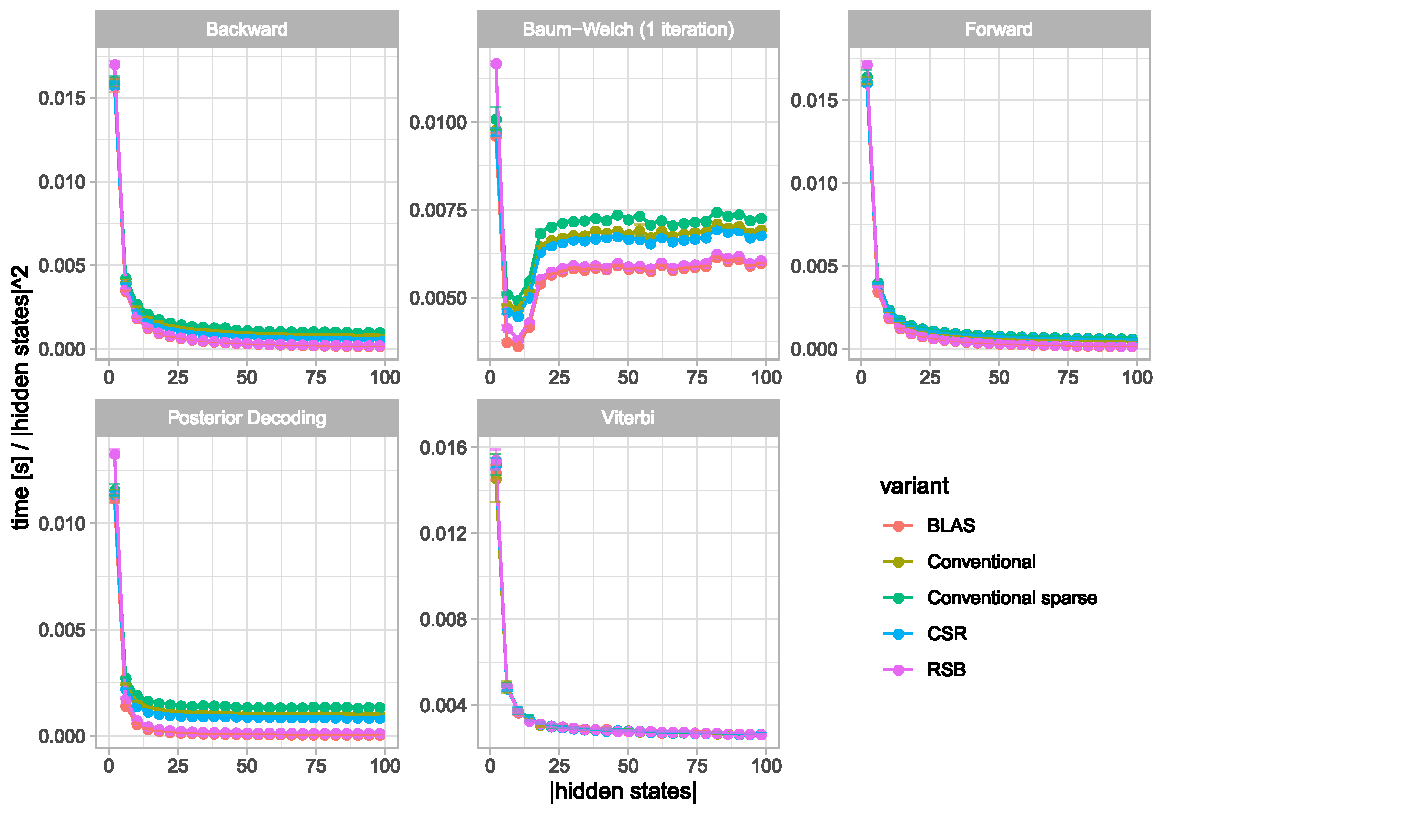
\includegraphics[scale=0.85]{figures/figure_C3_scaled.pdf}
    \caption{Running time of increasing number of hidden states for all algorithms and all implementations. Time measurement is averaged over 3 replicates. Error bars indicate standard deviation. Alphabet size = 4, input size = 100'000.}
    \label{app:hiddenstates}
\end{figure}




\begin{figure}[H]
    \centering
    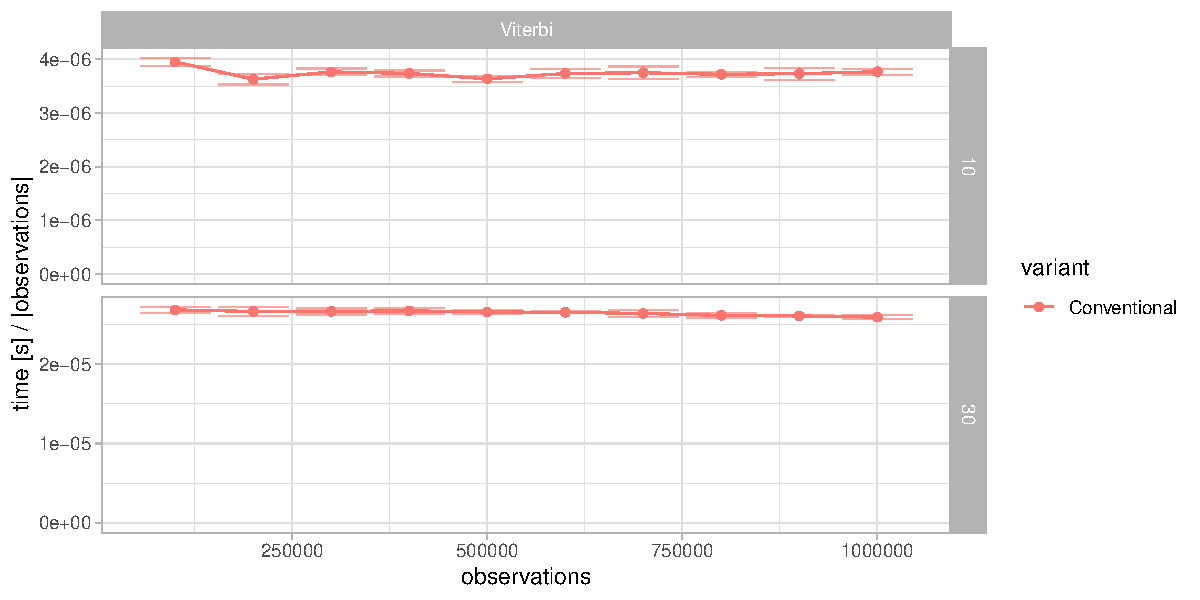
\includegraphics[scale=0.85]{figures/figure_A3_scaled.pdf}
    \caption{Running time of increasing number of observations in the Viterbi algorithm. For 10 and 30 hidden states. Time measurement is averaged over 3 replicates. Error bars indicate standard deviation. Alphabet size = 4. }
    \label{app:viterbi}
\end{figure}